\section{Iteración 3}

% Aquí va el desarrollo de la página web

Con el prototipo del sistema experto desarrollado el siguiente paso fue
proporcionar una interfaz amigable para el usuario a la par que accesible
desde cualquier lugar.

Para ello lo primero fue crear unos bocetos sobre el diseño que se quería tener
en la web. La idea original es que esta se componga de una página
principal en la que se explique el objetivo de la página y cual es su propósito.

Por otro lado tendremos dos secciones que se diferencien la una de la otra, de las
cuales una de ellas estará destinada a una versión rápida del sistema de apoyo mientras
que la otra será una versión mas exhaustiva. De este modo nos podremos adaptar
a las diversas situaciones en las que se puede utilizar la herramienta.
La primera será para aquellas situaciones en las que tenemos menos de un minuto
para que nos de un resultado. La segunda será para cuando podamos analizar
los resultados e introducir las variables con mayor calma puesto que no
tendremos prisa para ello.

Los resultados los bocetos se pueden ver en las figuras \hyperref[fig:Boceto página llenar]{5.7} y \hyperref[fig:Boceto página guiado]{5.8}.

\begin{figure}[htb]
  \centering
    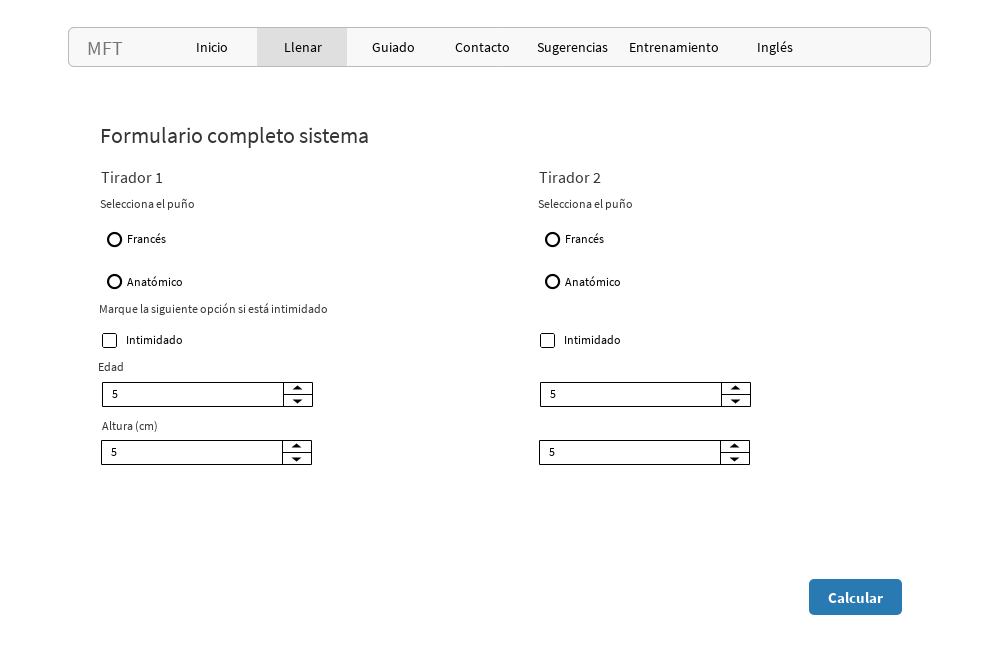
\includegraphics[width=0.8\linewidth]{bocetos/llenar}
  \caption[Boceto página llenar]{Boceto página llenar}
  \label{fig:Boceto página llenar}
\end{figure}

\begin{figure}[htb]
  \centering
    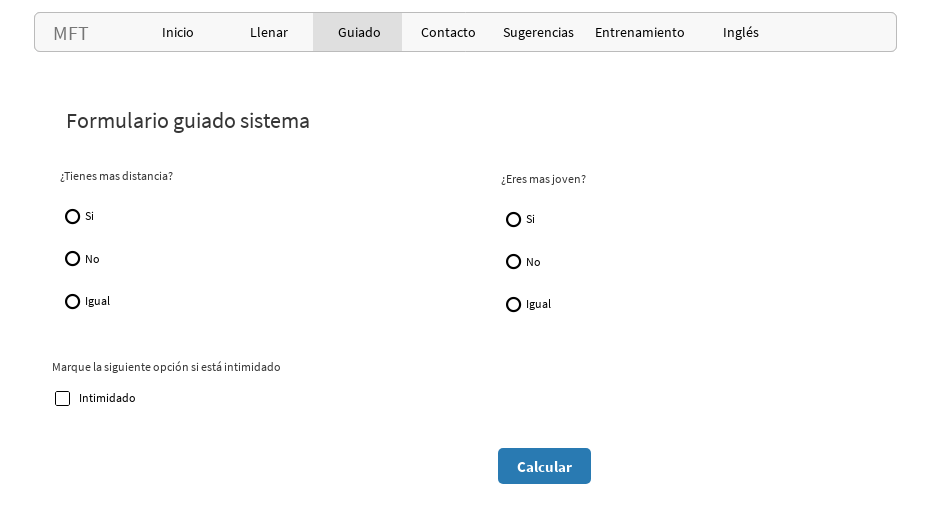
\includegraphics[width=0.8\linewidth]{bocetos/guiado}
  \caption[Boceto página guiado]{Boceto página guiado}
  \label{fig:Boceto página guiado}
\end{figure}

El resto de bocetos se pueden consultar en el \hyperref[cap:Bocetos]{anexo F}.

Una vez con los bocetos claros se decidió que tecnologías usar. Para el desarrollo
de la aplicación se decidió usar Ruby puesto que es uno de los lenguajes
de programación mas utilizados para el desarrollo rápido de aplicaciones web.
Otro de los motivos para escoger dicho lenguaje es el conocimiento obtenido
por el desarrollador en dicho lenguaje, de este modo no tendremos que añadir
tiempo de aprendizaje al proyecto, lo cual ahorrará recursos. En este caso el
recurso será el tiempo que tarde en aprender el nuevo lenguaje.

El paradigma utilizado será Modelo-Vista-Controlador. Siendo este el que más
favorece a la mantenebilidad del proyecto, permitiendo la ampliación de requisitos
del mismo mediante modelos para después ampliar a usuarios, perfiles de tiradores,
etc.

El desarrollo de la aplicación web se hizo en local, utilizando las herramientas
que proporciona ruby para ello. Además se utilizó control de versiones con un repositorio
el cual puede ser consultado en el siguiente enlace \url{https://github.com/grego1201/MFT-WEB}
o siguiendo el QR situado en la \hyperref[fig:Código QR repositorio web]{figura 5.9}.

\begin{figure}[htb]
  \centering
  \scalebox{.3}{
\includegraphics[width=0.8\linewidth]{QRWeb}}
  \caption[Código QR repositorio web]{Código QR repositorio web}
  \label{fig:Código QR repositorio web}
\end{figure}

Para ello se siguieron los siguientes pasos:

\begin{enumerate}
  \item \textbf{Inicialización:} Lo primero de todo será inicializar el proyecto.
    Hay muchos ejemplos de como inicializar un proyecto en ruby pero se siguió
    la documentación\footnote{\url{https://guides.rubyonrails.org/getting_started.html}} que te da la propia página web de ruby. Con esto tendremos
    lo básico para poder empezar a desarrollar la aplicación e ir añadiendo todo
    aquello que necesitemos.

  \item \textbf{Creación controladores:} Crearemos los primeros controladores de
    la aplicación que serán los mas importantes puesto que serán los encargados
    de manejar las peticiones hechas a las dos partes principales de la aplicación.
    Estos son los controladores para el apartado guiado y el completo. Además
    en este paso añadiremos los formularios en las vistas de dichos controladores
    de modo que podamos hacer las primeras pruebas.

  \item \textbf{Creación servicio toma decisión:} Crearemos un servicio que será
    encargado de toda la lógica del sistema de apoyo a la toma de decisión. Aquí
    nos encargaremos de trasladar todo el conocimiento obtenido anteriormente
    a una clase que tenga toda la lógica de modo que este servicio sea accesible
    por toda la aplicación. Además en este apartado añadiremos los correspondientes
    test para comprobar que la implementación ha sido la adecuada.

  \item \textbf{Creación vista resultados:} Daremos visualización a los resultados
    obtenidos por el servicio de toma de decisiones. De esta forma el usuario podrá
    ver cual es el resultado de dicho sistema.

  \item \textbf{Añadir bootstrap:} Añadiremos el framework bootstrap para ayudarnos
    a la aplicación de estilos en la página. De esta manera mejoraremos la usabilidad de la misma.

  \item \textbf{Añadir traducciones:} Haremos los cambios necesarios para permitir
    a la aplicación traducciones en distintos idiomas de forma que se pueda
    internacionalizar. En esta primera iteración se añadirá castellano e inglés.

  \item \textbf{Añadir página de inicio:} Crearemos la página de inicio en la que
    daremos información general de la aplicación, cual es su objetivo y de donde nace.

  \item \textbf{Añadir página de contacto:} Crearemos una página de contacto en la que
    se dará información de los responsables del proyecto y donde encontrarles.

  \item \textbf{Añadir página de sugerencias:} Crearemos una página en la que los usuarios
    podrán plasmar sus sugerencias de modo que la página y el sistema tenga retro-alimentación
    y así perfeccionarlo.

  \item \textbf{Añadir página entrenamiento:} Se añadirá un apartado en la página cuyo destino
    será que los tiradores puedan consultarla y obtener ideas de entrenamiento. Al principio
    tendrá una serie de acciones con un seleccionador de estas aleatorio y así que puedan
    practicarlas forzando a realizar dichas acciones.

  \item \textbf{Definir y añadir estilos:} Se definirán los estilos de los formularios, botones,
    textos, etc de la aplicación.
\end{enumerate}

Para asegurar la calidad de código se van a seguir dos principios. Estos son comprobar
el código con test y estos deberán cubrir un mínimo de 90\% de líneas de un fichero.
También seguiremos una guía de estilos. Esto nos asegurará en un futuro que todo el mundo
escriba el código de una forma \enquote{parecida}. Al menos seguirán unas reglas las cuales
no se podrán saltar. Entre ellas estará el número máximo de caracteres por línea,
número máximo de líneas por método, complejidad máxima de un método, etc.

Para lo primero se usará la gema \textit{simplecov}\footnote{\url{https://github.com/colszowka/simplecov}} la cuál nos permite configurar
los test de manera que luego genere un informe que se podrá consultar desde el navegador
en local. Un ejemplo del informe se puede ver en la \hyperref[fig:Ejemplo informe cobertura código]{firgura 5.10}.
En él se puede observar como se obtuvo una cobertura de código del 96.64\%. Esto deberá ser
mejorado en un futuro siendo el 100\% lo idóneo.

\begin{figure}[htb]
  \centering
  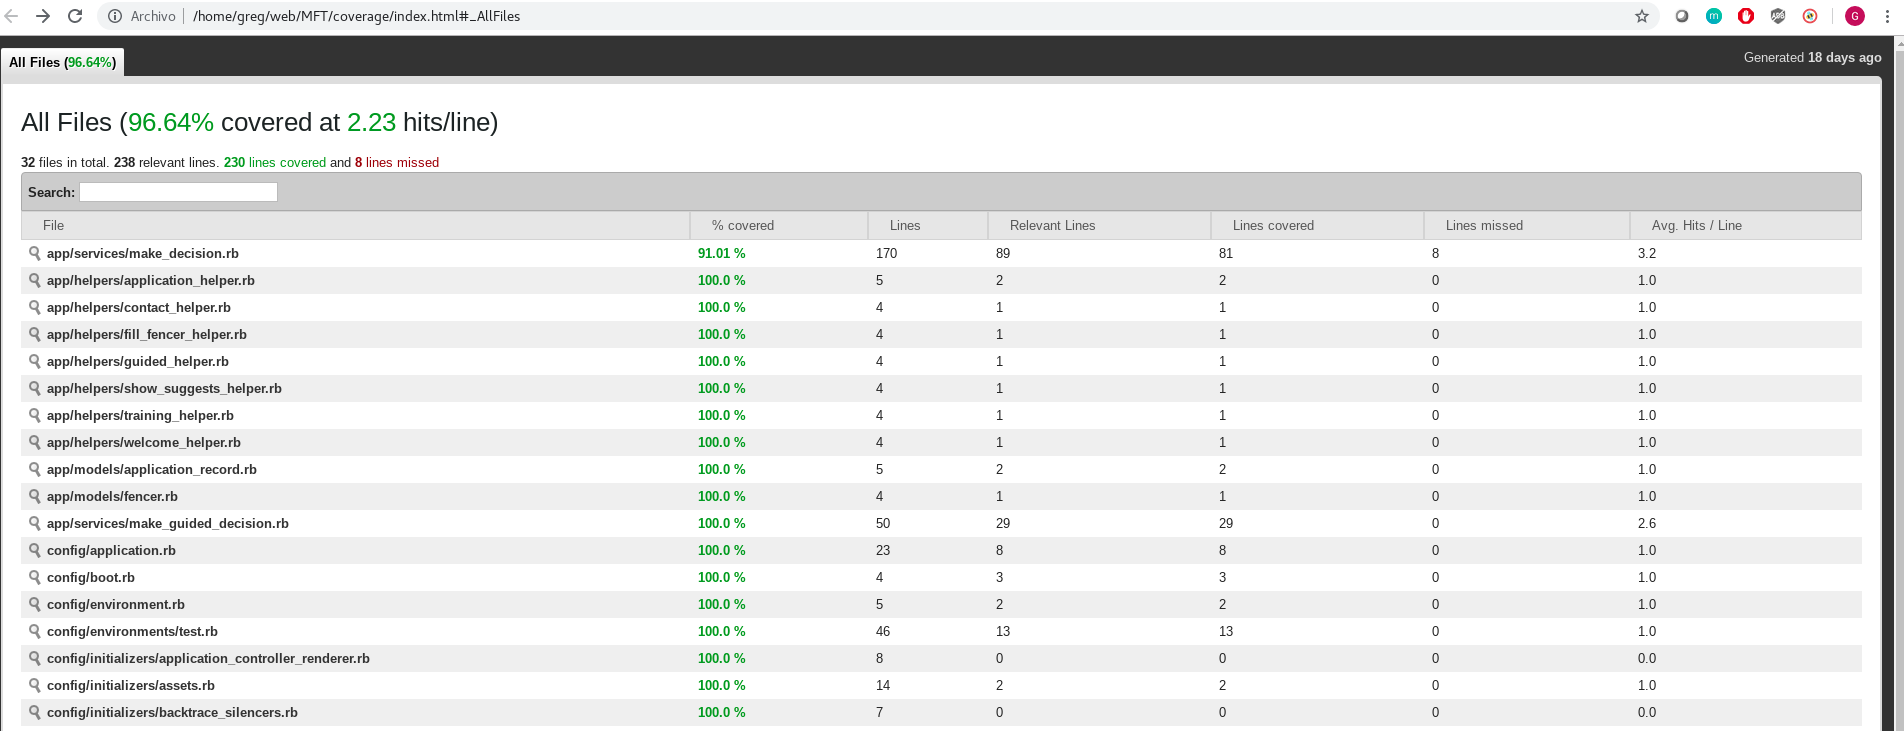
\includegraphics[width=1\linewidth]{simplecov}
  \caption[Ejemplo informe cobertura código]{Ejemplo informe cobertura código}
  \label{fig:Ejemplo informe cobertura código}
\end{figure}

En cuanto a la calidad de código se usó la librería rubocop\footnote{\url{https://github.com/rubocop-hq/rubocop}}. Esta te permite
fijar unas reglas de código mediante y después comprobar que estas se han cumplido.
Muchos editores tienen plugins para comprobar dichas normas fijadas en el proyecto
a la vez que escribes el código. Para este proyecto se cambiaron las normas por defecto
adaptandolas a las necesidades de este. Las modificaciones hechas fueron las siguientes:

\begin{itemize}
  \item \textbf{Longitud máxima de línea}. Este fue modificado para aumentarlo a 120 caracteres.
  \item \textbf{Longitud máxima de método}. Este fue modificado para aumentarlo a 15 líneas.
  \item \textbf{Longitud máxima de clase}. Este fue modificado para aumentarlo a 140 líneas.
  \item \textbf{Complejidad máxima}. Este fue modificado para aumentarlo a 21.
\end{itemize}

Con todo esto ya terminado podremos pasar al siguiente paso que será
dar acceso a la aplicación a cualquier persona que tenga acceso a internet.
